\section{PostBOUND - PostgreSQL Extension}
\label{sec:PostBound}

\begin{figure}[tb]
	\centering
	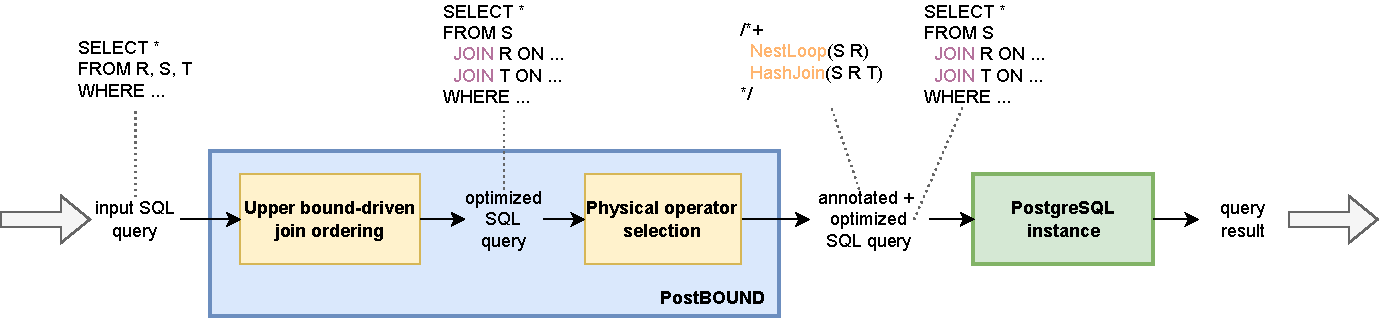
\includegraphics[width=0.95\linewidth]{figures/postbound-workflow-rework.pdf}
	\caption{The basic \emph{PostBOUND} query optimization workflow.}
	\label{fig:postbound-workflow}
\end{figure}

In this section, we present \emph{PostBOUND}, our developed framework to seamlessly integrate upper bound-driven optimization of SPJ queries into PostgreSQL.
At its core, \emph{PostBOUND} consists of two components as depicted in Fig.~\ref{fig:postbound-workflow}, which are completely implemented in Python: 
First, for each incoming SQL query, the \texttt{join ordering component} determines an optimized join order that is used for query execution. 
The underlying process applies a generalized and extensible implementation of our UES concept (see Section~\ref{sec:UES}). 
The output of this first component is a rewritten SQL query with an explicit join order.
Secondly, our subsequent \texttt{physical operator selection} component enforces the usage of individual physical join and base table scan operators. 
The resulting query annotations to enforce physical operators are used together with the rewritten SQL of our first component to execute the query with an arbitrary PostgreSQL instance.
With this approach, the join order as well as the physical operator selections are fixed by \emph{PostBOUND} using an upper bound-driven optimization concept. 
Implementation details of both components are described in the following sections\footnote{ 
Although \emph{PostBOUND} is currently tailored to PostgreSQL, it can be adapted to other database systems and we plan to integrate different backends in the near future.}.

\subsection{Upper Bound-driven Join Ordering Component}
\label{sec:postbound-join-ordering}


The upper bound-driven join ordering is the first component of \emph{PostBOUND} and it focuses on a robust join sequence in order to prevent disastrous execution plans.
The main goal of this component is to optimize the join order of an arbitrary SQL query by transforming implicit joins like \sql{SELECT * FROM R, S, T WHERE ...} into an explicit ordering via \sql{JOIN} clauses, such as \sql{SELECT * FROM S JOIN R ON ... JOIN T ON ...}. During query execution, PostgreSQL provides means to enforce such an ordering of \sql{JOIN} statements.
Fig.~\ref{fig:postbound-interaction} shows the general steps involved in this process:
First, a \emph{join graph} is constructed by parsing the incoming SQL query.
This graph serves as the central data structure for optimization and describes the role each table plays in the query. 
We apply the same distinction between n:m joined tables and primary key joined tables, as originally proposed in UES~\cite{hertzschuch-21-ues}.
Based on this graph, the actual optimization loop is executed in the \texttt{join graph enumerator}. 
During each iteration, the algorithm pulls n:m candidate tables from the join graph and evaluates their current upper bounds, such that the candidate with minimum bound is inserted into the join tree (tables colored in orange in Fig.~\ref{fig:postbound-interaction}).
This selection focuses only on n:m joined tables, because primary key/foreign joins are again treated as special filters of the foreign key (and by extension n:m joined) table that can potentially lower the candidate's upper bound.
Therefore, primary key tables are inserted into the join tree together with their foreign key counterpart. 
Again, following the UES philosophy, the join between the candidate table and its primary key partners can be executed as a subquery, as the enumerator sees fit (see below for details).
Once all tables of the join graph have been included in the join tree, the rewritten query with an explicit join order syntax is constructed based on the derived optimal join order.

\begin{figure}[tb]
	\centering
	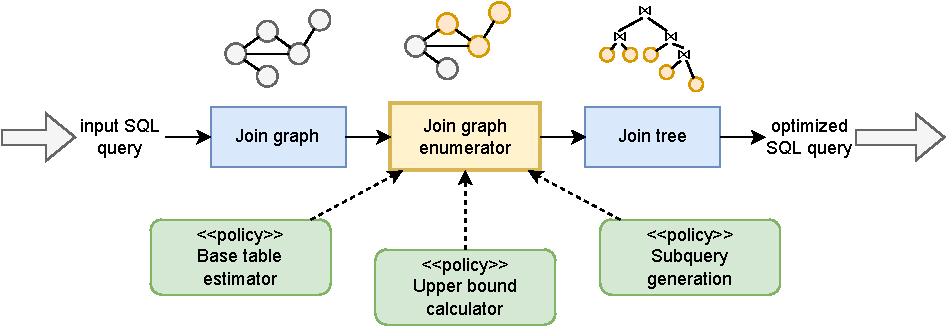
\includegraphics[width=0.95\linewidth]{figures/postbound-interaction-rework.pdf}
	\caption{Interaction between the core \emph{PostBOUND} components for join ordering.}
	\label{fig:postbound-interaction}
\end{figure}

In \emph{PostBOUND} we expand on the original UES algorithm in two ways: On the one hand, this entire enumeration process can be adapted with custom policies to modify specific aspects of its behavior. These policies include:

\begin{compactitem}
    \item[\textbf{Base table estimates:}] The \texttt{join ordering} component of \emph{PostBOUND} does not require a specific strategy to estimate the number of tuples in a (filtered) base table. It only relies on the existence of a numerical estimate and makes no assumption about how it is obtained. Nevertheless, three basic strategies are already provided and new strategies can be injected easily. The provided strategies include: (i) delegating the estimation process to the PostgreSQL-native optimizer, (ii) sampling a fraction of the filtered table, or (iii) executing the entire filter predicate and counting the result tuples.
    \item[\textbf{Upper bound calculation and statistics:}] To obtain upper bounds of join cardinalities, different strategies have been proposed in recent literature~\cite{DBLP:conf/sigmod/CaiBS19,DBLP:journals/corr/abs-2201-04166,hertzschuch-21-ues}. \emph{PostBOUND} does not restrict the choice of any particular formula, as long as it is capable of the calculation of an upper bound of any $n$-ary join. Currently, the UES formula (see Section~\ref{sec:UES}) and two variations (see Section~\ref{sec:TighterBounds}) are provided with \emph{PostBOUND}. Since join upper bound calculation oftentimes relies on specific \emph{statistical information}, each calculation strategy ships its own tailored implementation. The statistics interface receives update information from the optimization loop.
    \item[\textbf{Subquery generation:}] \label{item:postbound-subqueries} Lastly, the \texttt{join ordering} component of \emph{PostBOUND} also delegates the decision when to generate subqueries for primary key/foreign key joins to custom policies. In this case, four strategies are already supplied by default: (i) a greedy strategy that always generates subqueries, (ii) a defensive strategy that generates subqueries if they guarantee to reduce the size of the foreign key table (as proposed in \cite{hertzschuch-21-ues}), (iii) a ``smart'' strategy that generates subqueries if a reduction below a certain threshold is guaranteed (which is a generalization of strategy (ii)), and finally, (iv) a strategy that never generates subqueries at all, thereby leaving all join paths linear.
\end{compactitem}

On the other hand, the entire enumeration process is mainly tailored to SPJ queries containing a mixture of n:m and primary key/foreign key joins. 
To broaden this scope, if an incoming SQL query does not match this structure, it will be handled by specialized procedures:

\begin{compactitem}
    \item[\textbf{Primary key/foreign key queries:}] To optimize queries that do not contain any n:m join -- such as queries on star- or snowflake schemas -- a heuristic approach inspired by UES is used. In this case and since primary key/foreign key joins are bound to never produce more tuples than the cardinality of the foreign key relation, our enumeration algorithm starts with the smallest foreign key table and iteratively includes connected tables according to their respective cardinality estimates. This strategy tries to minimize the number of tuples that have to be processed, but only treats the join order as a local optimization problem. An extension that also considers the join cardinalities could be a natural and effective improvement in future work.
    \item[\textbf{Cross product queries:}] Queries with cross products are characterized by tables that are neither directly nor indirectly linked with join predicates. Using the join graph, this situation can be easily detected through the existence of multiple graph components. Since each of these components represents a complete join graph on its own, an optimized upper bound-driven join order can be obtained per partition. Afterwards, a final join order can be constructed by sorting the individual join trees according to their upper bounds.
    \item[\textbf{Composite join predicates:}] In contrast to the two previous extensions, composite join predicates do not influence the join order itself. Rather, composite join predicates need to be handled during the upper bound calculation and are, thus, subject to the policies. However, they still constitute a special case that needs to be considered to ensure independence from specific workloads. Therefore, they are quickly discussed here. For upper bound-driven calculation, composite join predicates can be handled quite naturally: Since a conjunctive predicate requires each of the individual base predicates to be fulfilled, the final upper bound is constrained by the smallest estimate of the base predicates. Thus, the upper bound approach can simply calculate the minimum of base estimates. Other upper bound approaches may rely on different strategies such as the calculation of mean bounds, but for UES as well as the two presented variants in Section~\ref{sec:TighterBounds}, the minimum strategy is used.
\end{compactitem}

Based on these extensions, \emph{PostBOUND} is currently capable of optimizing SPJ queries, as well as some non-SPJ queries, as long as the following requirements are met: (i) each part of the \sql{SELECT} clause is either directly derived from a base attribute or an aggregation of such attributes, (ii) all joins are either equality predicates over base table attributes, or conjunctions of such predicates, (iii) each base table can optionally be filtered using arbitrary predicates that are not optimized further, and (iv) each query can optionally contain a \sql{GROUP BY}, \sql{ORDER BY}, or \sql{HAVING} clause, which are also ignored during optimization. These restrictions are mostly due to technical reasons to keep the implementation effort manageable, rather than being caused by limitations of the underlying ideas.


\subsection{Physical operator selection component}
\label{sec:postbound-operator-selection}

For an efficient query execution, not only the join order is important, but also the selection of the best-fitting physical operators~\cite{DBLP:journals/pvldb/HertzschuchHHL22}. 
In \emph{PostBOUND}, this selection process is handled by a dedicated \texttt{physical operator selection} component (cf. Fig.~\ref{fig:postbound-workflow}). 
Although many state-of-the-art query optimizers intertwine the operator selection and the determination of the optimal join order, the upper bound approach makes this difficult due to the overestimation as shown in Fig.~\ref{fig:UESOverestimationJOB}. Therefore, new, specific approaches are required. 
In~\cite{DBLP:journals/pvldb/HertzschuchHHL22}, we have recently presented such a selection approach using a learning-based concept that allows physical operator decisions for arbitrary join paths based on learned query feedback.
Other approaches are also conceivable and thus, we decided to provide a specific component in \emph{PostBOUND} to accommodate such selection approaches. 

Since forcing the execution of joins or table scans with specific algorithms depends strongly on the concrete database system, \emph{PostBOUND} focuses on two means supported by PostgreSQL. 
The first strategy uses runtime variables that modify the behavior of the PostgreSQL planner. 
For example, the \mbox{\sql{SET enable\_nestloop = 'off';}} option used by UES disables nested loop joins globally for all following queries in a workload. 
Secondly, \emph{PostBOUND} also provides interfaces that force individual joins to be executed with specific operators. 
This feature is based on the \emph{pg\_hint\_plan}\footnote{\url{https://github.com/ossc-db/pg_hint_plan/}} extension that specifies a number of \emph{query hints}. 
A hint is essentially a comment preceding an SQL query that modifies the execution and optimization behavior of PostgresSQL for that specific query. 
For example, the hint \sql{/*+ HashJoin(movies actors) */} would enforce the join between \sql{movies} and \sql{actors} to be executed by a Hash join. 
How these hints are generated is left to user-specific selection strategies. 
In our ongoing research, we want to generate query hints for joins based on upper bounds, which however requires tighter upper bounds. One approach to infer such bounds is presented in the following section.

%\subsection{Summary}
%\label{sec:postbound-summary}

%\emph{PostBOUND} is our framework to systematically evaluate different approaches to pessimistic query optimization. \emph{PostBOUND} is a PostgreSQL-specific set of components that use a query optimization algorithm inspired by UES. The algorithm enables the adaption of base table estimates, join cardinality estimates and the generation of subqueries. Furthermore, \emph{PostBOUND} is designed to operate without any additional user-supplied data and fetches all required information from the Postgres instance. This enables independence from specific benchmarks and database schemas. Using this framework, we can optimize different workloads and compare their results in a reproducible and transparent way.
